% !TEX encoding = UTF-8 Unicode
\documentclass[a4paper]{article}

\usepackage{color}
\usepackage{url}
\usepackage[T2A]{fontenc} % enable Cyrillic fonts
\usepackage[utf8]{inputenc} % make weird characters work
\usepackage{graphicx}
\usepackage{fancyhdr}
\usepackage{amsmath}
\usepackage{tablefootnote}

\usepackage[english,serbian c]{babel}

\usepackage[unicode]{hyperref}
\hypersetup{colorlinks,citecolor=green,filecolor=green,linkcolor=blue,urlcolor=blue}

\usepackage{listings}

\usepackage[a4paper, total={6in, 8in}]{geometry}

%\newtheorem{primer}{Пример}[section] %ćirilični primer

\definecolor{mygreen}{rgb}{0,0.6,0}
\definecolor{mygray}{rgb}{0.5,0.5,0.5}
\definecolor{mymauve}{rgb}{0.58,0,0.82}

\lstset{ 
  backgroundcolor=\color{white}, 
  basicstyle=\scriptsize\ttfamily, % the size of the fonts that are used for the code
  breakatwhitespace=false,         % sets if automatic breaks should only happen at whitespace
  breaklines=true,                 % sets automatic line breaking
  captionpos=b,                    % sets the caption-position to bottom
  commentstyle=\color{mygreen},    % comment style
  deletekeywords={...},            % if you want to delete keywords from the given language
  escapeinside={\%*}{*)},          % if you want to add LaTeX within your code
  extendedchars=true,              % lets you use non-ASCII characters; for 8-bits encodings only, does not work with UTF-8
  firstnumber=1000,                % start line enumeration with line 1000
  frame=single,	                   % adds a frame around the code
  keepspaces=true,                 % keeps spaces in text, useful for keeping indentation of code (possibly needs columns=flexible)
  keywordstyle=\color{blue},       % keyword style
  language=Python,                 % the language of the code
  morekeywords={*,...},            % if you want to add more keywords to the set
  numbers=left,                    % where to put the line-numbers; possible values are (none, left, right)
  numbersep=5pt,                   % how far the line-numbers are from the code
  numberstyle=\tiny\color{mygray}, % the style that is used for the line-numbers
  rulecolor=\color{black},         % if not set, the frame-color may be changed on line-breaks within not-black text (e.g. comments (green here))
  showspaces=false,                % show spaces everywhere adding particular underscores; it overrides 'showstringspaces'
  showstringspaces=false,          % underline spaces within strings only
  showtabs=false,                  % show tabs within strings adding particular underscores
  stepnumber=2,                    % the step between two line-numbers. If it's 1, each line will be numbered
  stringstyle=\color{mymauve},     % string literal style
  tabsize=2,	                   % sets default tabsize to 2 spaces
  title=\lstname                   % show the filename of files included with \lstinputlisting; also try caption instead of title
}

\begin{document}

\title{
\textbf{\LARGE{Родна (не)равноправност у информатици у Србији}}\\
\vspace{10}
\small{Семинарски рад у оквиру курса\\Методологија стручног и научног рада\\ Математички факултет у Београду}}

\author{Катарина Милошевић,  Тамара Јевтимијевић, Анђела Ђуровић \\ 
        \textit{mi231019@alas.matf.bg.ac.rs}, \textit{mi231045@alas.matf.bg.ac.rs}, 
        \textit{mi231024@alas.matf.bg.ac.rs} \\\\
        \textit{професор:} др Милена Вујошевић Јаничић}

\date{Новембар 2023.}

\maketitle
\thispagestyle{empty}

\renewcommand{\abstractname}{Сажетак}

\abstract{
Родна равноправност подразумева једнаке могућности, једнаку видљивост и једнаку заступљеност
мушкараца и жена у свим сферама приватног и јавног живота. 
Овај рад започећемо са историјским освртом на питање родне равноправности
у информатици, а затим ћемо се бавити анализом исте теме у Србији, за разне подобласти. Иако
је ово област којом су некада доминирале жене, данас је то поприлично другачије. 
На самом крају биће речи о заједницама које се баве промовисањем родне равноправности у Србији, 
као и које се то иницијативе баве родном равноправношћу и шта су циљеви тих иницијатива.
}

\tableofcontents

\section{Увод}
\label{sec:uvod}

Протеклих година пратимо убрзан развој ИКТ\footnote{Информационо-комуникационе технологије.} 
индустрије, како у свету, тако и у Србији. Живимо у времену у коме технологија прожима сваки, па и
најмањи део наших живота, у времену у коме је готово немогуће замислити дан, па чак и сат, 
проведен без употребе рачунара и мобилног телефона како на послу, тако и у приватном животу. 
Поставља се питање да ли овај развој прате подједнако жене и мушкарци? \\
Оно што је сигурно то је да се све већи број младих у Србији одлучује за факултете информатике, 
рачунарства и математике. Показује се да последњих година број жена у ИТ свету јесте у порасту, а 
све већи број студенткиња опредељује се за смерове информатике и рачунарства. Мит о 
жени у ИТ окружењу, као области која је резервисана искључиво за мушкарце, не постоји у оној мери,
у којој је постојао пре неколико година. Мада и поврх свега тога, статистике још показују да, и 
даље у овој области, постоји неравноправност полова. 

\subsection{Родна равноправност у информатици кроз историју}

Иако се данас, на основу доступне статистике, може закључити да је информатика првенствено „мушка”
област, историјски ово није било тако. Саме почетке информатике и рачунарских наука обележиле су 
жене. Многе од њих неправедно су заборављене, те се зато данас стиче утисак да се однос
полова у информатици није мењао кроз време. \\

Током четрдесетих и педесетих година XX века програмирање се сматрало женским послом. Више жена 
уписивало jе рачунарске факултете, него медицину, хемиjу, право и сл. У часопису "Космополитен" 
(Cosmopolitan - The Women's magazine) 1967. године изашао je чланак под насловом "Девојке 
рачунарства". У њему се програмирање ставља раме уз раме са пословима коjе су традиционално 
обављале жене, као што су секретарица, учитељица, социjална радница и сл.
У то време мушкарци су се бавили више хардвером, а жене софтвером и због тога се софтвер сматрао 
мање престижном облашћу \cite{women_softver}. Постепено jе проценат жена у овом сектору опао, 
поготово 80. година поjавом првих рачунара опште намене, коjи су постали доступни домаћинствима. 
Рачунари су се промовисали као играчке за дечаке или одличне направе на коjима мушкарци могу да 
раде. На тај начин jе програмирање за дечаке и мушкарце вештачки креирано кроз рекламе.\\

Историjски гледано, тек последњих децениjа jе у програмирању већи удео мушкараца у односу на жене.
До тад су жене доминирале у овом пољу. Заправо, први програмер у свету била jе жена Ада Лавлеjс 
(Ada Lovelace 1815 - 1852) \cite{ada_l}. Са 17 година упознала је Чарлса Бебиџа 
(Charles Babbage 1791 - 1871), са којим је заједно радила на нацрту за диференцијалну машину, као 
и за аналитичку машину, за коју је у 19. веку написала први алгоритам \cite{ada_l_prog}. Сваке 
године се широм света обележава њен дан (други уторак октобра), како би се признали и прославили 
доприноси жена у науци, технологиjи, инжењерингу, информатици, рачунарству и математици. 

Након Америчког грађанског рата, жене су запошљаване као „људски рачунари” и то најчешће удовице,
док су остале добијале прилику тек када је фалило мушке радне снаге. Биле су мање плаћене него 
мушкарци, док су неке чак и волонтирале, иако су биле једнако способне \cite{women_lover_price}. 
Временом су жене почеле и да се школују за рачунарске послове, те је њихов број у овој области 
непрестано растао \cite{women_education_it}.\\

\newpage
Крајем шездесетих година прошлог века наступиле су велике промене у односу полова у програмирању. 
Број жена је и даље био значајан, али су биле знатно мање плаћене \cite{women_education_it, 
women_price}. Према неким ауторима, тестови, које су добијали пријављени за посао, били су 
намерно више прилагођени мушкарцима \cite{women_price}. Такође, креиране су видео игре пуне акције
тако да су примарно циљале мушарце, који су чинили већину корисника рачунара. Број жена 
у рачунарству достигао је врхунац средином 1984. године када је проценат женских дипломаца био 
37.1\%. Затим је уследио константан пад, где је већ 1998. тај број био 26.7\% 
\cite{women_procent}. У 21. веку ситуација се није много мењала, те је од почетка 2000. проценат 
женских дипломаца констатно испод 20\%. Покренут је велики број иницијатива и уложена огромна 
колична новца са циљем да се међу девојчицама и адолесценткињама промовишу рачунарске науке, са 
циљем да се јаз међу половима умањи \cite{smanjenje_jaza}. У сваком случају, ако се на основу 
историје нешто може закључити, то је да нема оправдања да се информатика сматра професијом 
предодређеном за било који од два пола, без обзира на статистичке податке.


\subsection{Родна равноправност у Србији}

Половину становника Србије чине жене (51,77\%), али је њихово учешће када се гледа запосленост 
43,67\%. Међутим, проценат жена, који је на високим позицијама, нагло опада. На месту 
руководилаца, функционера и законодаваца жене чине 29\%, чланова Владе 25\%, председника општина 
или градоначелника 7\% \cite{stat}. Како на државном нивоу доминирају мушкарци, тако доминирају и 
на многим другим пољима. Једно oд њих је и ИТ сектор.\\

Устав Србије, усвојен 2006. године, подржава равноправност жена и мушкараца, прописује политике 
једнаких могућности и забрањује директне и индиректне облике дискриминацијe. Године 2021. Србија 
је усвојила нови оквирни закон у области заштите права жена - \textit{Закон о родној 
равноправности}. Поред њега усвојени су и \textit{Закон о изменама и допунама} и \textit{Закон о 
забрани дискриминацијe}. Такође, донесена је и стратегија за превенцију и сузбијање родно 
заснованог и породичног насиља за период 2021-2025, као и нова национална стратегија - 
\textit{Стратегија за родну равноправност}. Иако постоје закони и политике, које промовишу родну 
равноправност, жене су недовољно заступљене у доношењу одлука у свим сферама друштвеног, 
економског и политичког живота Србије \cite{zakon1}. \\ 

На 26. Копаоник бизнис форуму потписан је документ о посвећености компанија родној равноправност.
Kомпаније, које су се окупиле око овог документа, деловаће у оквиру Алијансе за родну 
равноправност \cite{alijansa}. Главна замисао потписница документа је да се омогући да жене и 
мушкарци зарађују исто за исте послове, као и да се повећа број жена на високим позицијама, али и 
другим. Повод за окупљање компанија око заједничког циља било је истраживање које је спровела ИКЕА
у сарадњи са ИПСОСОМ, које је показало да је више од 50\% мушкараца свесно свог привилегованог 
положаја на радном месту у односу на жене, а да је свака седма жена доживела дискриминацију 
на радном месту.

Према истраживању Светске банке "Жене, бизнис и право" \cite{banka}, Србија је по основу једнаког 
правног статуса на 18. месту у конкуренцији од 188 земаља света и најбоље рангирана држава у 
региону. По другом истраживању вршеном од стране Светског економског фонда, Србија је 76. 
(од 149 земаља) по економској равноправности жена и мушкараца, а на 38. месту по индексу родне 
равноправности \cite{danas}.\\

И поред значајних напредака учињених на плану постављања правног оквира за постизање родне 
равноправности, ипак се намеће питање да ли је и у којој мери родна равноправност постигнута у 
пракси. Индекс родне равоправности за Србију показује да Србија није још ни на пола пута до 
постизања пуне родне равноправности, те да још пуно тога треба учинити како би се смањио 
родни јаз.  

\section{Однос полова у академији у информатици у Србији}

Иако стереотип да девојчице имају више проблема са математиком и даље постоји, 
истраживања показују да нема разлике у савладавању математике између девојчица 
и дечака \cite{stereotip}. Јачина овог стереотипа ствара изазове у остваривању 
пуног потенцијала девојчица и утиче на самопоуздање. Чак и жене, које имају 
афинитете и занима их технологија, ће имати одступницу и неће хтети да се упусте 
у технологију из страха да не потврде стереотип: "Жене нису за ИТ".\\

Високе школе и факултете више уписују и завршавају жене, показују подаци Републичког 
завода за статистику. Међу уписаним студентима жена је 2019. године било 57\%,
а међу дипломираним 59\% \cite{zene_i_musk_u_Srb}. Ипак, није у свим областима присутна једнакост.

Према извештају Међународне организације рада, број жена у Србији са универзитетским 
дипломама у МИНТ\footnote{Математика, Инжењерство, Наука и Технологија} пољима је 43\%.
Само у пољу математике је више жена него мушкараца, али разлог за то је што се 
жене опредељују да предају у школама. У инжењерству их има мање од 40\%, а у 
технологијама не чине ни трећину. Према подацима Републичког завода за статистику академске 
2020/21. године у Србији су студенткиње чиниле нешто мање од једне трећине (30,8\%) укупног броја 
(23 061) оних који студирају ИКТ област, док су у области друштвених наука чиниле више од две 
трећине (66,3\%) од укупног броја студената (27.403) \cite{startup_infos}. Жене чине у просеку 
35\% дипломираних инжењера првог степена образовања и 42\% другог степена образовања 
\cite{vlada_ikt}.\\

Истраживање о заступљености жена међу дипломцима на Електротехничком факултету у Београду 
показује да је у периоду од 1923. године, кад је одбрањен први дипломски рад на 
ову тему, па све до 2010. године било око 18\% жена у односу на укупан број 
(око 20 000) оних које су стекле диплому. До ових резултата дошле су доц. др Надица 
Миљковић са Електротехничког факултета и доц. др Биљана Станковић са Филозофског факултета. С 
ведрије стране, према подацима београдског Електротехничког факултета број девојака, које полажу 
пријемни на њиховом факултету из године у годину расте, а тај позитиван тренд почео 
је 2011. године, када је број девојака пријављених за пријемни био 20\%. 
Само 2018. године број уписаних девојака прешао је једну трећину укупног броја студената на ИТ 
смеровима. Иако овај раст није драматичан, позитивно је видети да се број девојака, које се 
интересују за техничке науке и софтверско инжењество из године у годину повећава и да постоји 
позитиван тренд раста заступљености девојака/жена у ИТ свету.

\section{Однос полова у индустрији у информатици у Србији}

ИКТ се развијајају веома брзом динамиком, а у овом сектору се тиме отварају нове могућности за 
запошљавање. Са друге стране, подаци показују да жене чине мање од 20\% стручњака у ИКТ сектору. 
Ови подаци говоре колико је важно радити на обуци жена и проширивању њихових ИКТ знања, промоцији 
ИКТ-а, као и мотивасању жена да се професионално баве ИКТ-ом. Предности ИКТ-а за жене су 
многобројне и омогућавају решавање великог броја питања на пољу родне равноправности, од смањења 
сиромаштва, превазилажења изолације жена, давање гласа женама до генералног побољшања родне 
равноправности \cite{vlada_ikt}. Оснаживање жена путем ИКТ-а директно је повезано са социјалним и
економским развојем, те данас представљају најмоћније алате за повећање приступа жена образовању, 
здравству и финансијским услугама. Ови фактори утичу на побољшање квалитета живота жена и њихових 
породица, а самим тим и друштва у целини. \\

У Србији су 2020. жене чиниле 25\% ИТ стручњака, што је за 6,5\% више него 2011. године 
\cite{danas_it}. Резултати истраживања показују да у ИТ заједници преовлађују мушкарци, они 
узраста 18 - 39 година, са стеченим вишим или високим образовањем. Према резултатима, мушкарци 
имају просечно веће плате него жене (1677 EUR наспрам 1277 EUR). Најчешћа плата код мушкараца је 
1000 EUR , док је код жена упола мања и износи 500 EUR \cite{puls_srpske_it}. Поред разлике у 
платама, постоје разлике и у разним областима послова. Те разлике приказане су на слици 
\ref{fig:odnosi}.

Према резултатима најновијег истраживања, под називом „Истраживање о улози ИКТ-а на положај жена 
на тржишту рада“, Министарства рада, запошљавања и социјалне политике, у Србији је мање од 20\% 
жена на руководећим положајима у ИТ предузећима, иако светска статистика показује да учешће жена 
на руководећим положајима доприноси позитивном финансијском успеху ИТ компанија.
Жене чине само 15\% менаџера и само 11\% стратешких експерата, али су уочљиво заступљене у 
категорији стручњака \cite{dijalog_it}. Оно што је очигледно, то је да жене знатно заостају за 
мушкарцима на пољу професионалног бављења информационо-комуникационим технологијама.\\

\begin{figure}[h!]
    \centering
    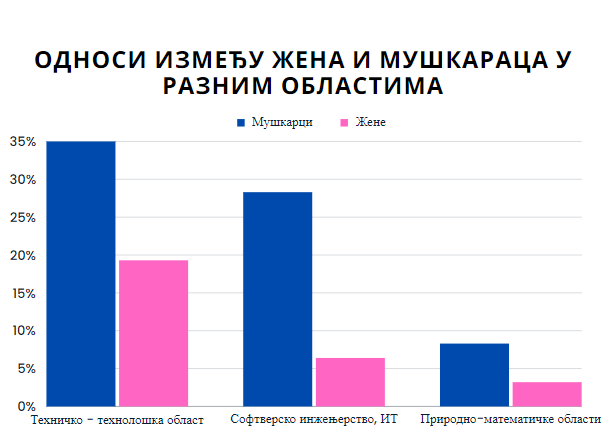
\includegraphics[width=0.8\textwidth, height=7cm]{Slike/odnos_oblasti.png}
    \caption{Односи између жена и мушкараца у разним областима \cite{zene_i_musk_u_Srb}.}
    \label{fig:odnosi}
\end{figure}

Проблем о ком се такође прича јесте тај што постоје незваничне информације да у неким фирмама у 
Србији, за исте позиције и завршене факултете, жене су биле плаћане мање од мушкараца. Оно што 
девојчице од малена могу да примете јесте да нема пуно женских великих узора у ИТ индустрији, чиме
нису охрабрене да крену тим путем. Поред ових прича и веровања да ће бити мање плаћене, како у 
страним државама тако и у Србији, жене често и одустају од овог занимања. 

Предрасуде и стереотипи отежавају достизање суштинске родне равноправности у
свим областима живота и рада па тако и у области науке, технологије, иновација
и информационо-комуникационих технологија (ИКТ). Светска истраживања показују
да су девојке и девојчице надарене и за техничка занимања и професије, али
се због притиска владајућих друштвених стереотипа и предрасуда да за жене
нису наука, технологија, иновације и информационо-комуникационе технологије,
радије одлучују за неке друге професије у друштвеним областима. Кључна је
промена свести јавности о штетном утицају владајућих друштвених стереотипа и
предрасуда о женама и мушкарцима у нашем друштву у свим областима живота
и рада, па тако и у претходно наведеним областима.
Ово је јако битно како би се обезбедило равноправно учешће и једнаке могућности и користи за 
оба пола у смислу усавршавања, економског оснаживања, рада и запошљавања у наведеним областима. \\

Занимљиво је да сва истраживања показују да компаније које међу својим запосленим имају једнак 
број запослених жена и мушкараца боље послују у односу на просек у својој индустрији за 15\%. 
Такође, компаније које у свом борду директора имају бар једну жену постижу боље резултате 
\cite{eu_it_sektor}.

Током истраживања ове теме у Теленору, дошло се до информациј да у Теленору ради приближно једнак 
број мушкараца и жена. Жене чине 48\% од укупног броја запослени, а на менаџерским позицијама ради
42\% жена. Сличан однос је и у самој управи компаније. Од осам чланова управе, три су жене. 
Занимљиво је да и сектор Технике, у којем ради највећи број ИТ стручњака, води жена 
\cite{telenor_it}. 
Подаци од стране компаније Вега ИТ показали су да су у Вега ИТ компанији преко 30\% запослених 
управо жене \cite{vega_it}.

\section{Однос полова у информатици у Србији у односу на свет}

Четвртину специјалиста информационо-комуникационих технологија у Србији чине жене, што је 
више од европског просека, према подацима Еуростата за 2020. годину. Жене су 2020. чиниле 18,5\% 
ИТ стручњака запослених у Европској унији. Њихов број је од 2011. растао брже него број мушкараца,
који раде у том сектору \cite{danas_it}. На слици \ref{fig:zene_i_muskarci_it} приказан је
однос између мушкараца и жена у ИТ свету у Европи. \\

\begin{figure}[h!]
    \begin{center}
        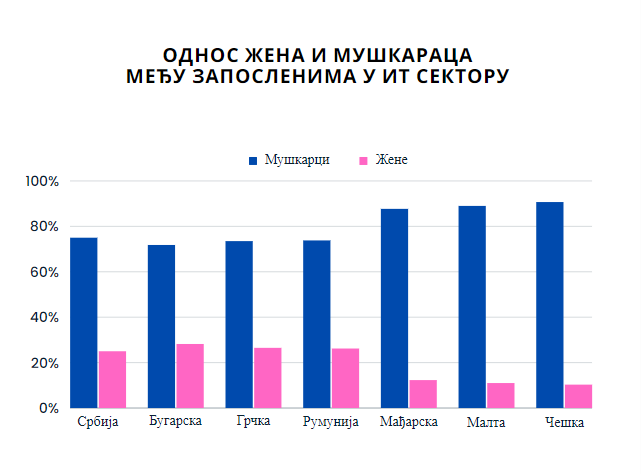
\includegraphics[width=0.8\textwidth, height=7.2cm]{Slike/odnos_muskaraca_i_zena.png}
    \end{center}
    \caption{Однос жена и мушкараца међу запосленима у ИТ сектору \cite{danas_it}.}
    \label{fig:zene_i_muskarci_it}
\end{figure}

\newpage
Када је у питању образовање, Србија има најмањи проценат специјалиста за ИКТ са високим 
образовањем међу земљама ван ЕУ (57,4\%) \cite{danas_it}. На слици \ref{fig:it_evropa} 
приказана је заступљеност ИТ стручњака у индустрији. 

\begin{figure}[h!]
    \begin{center}
        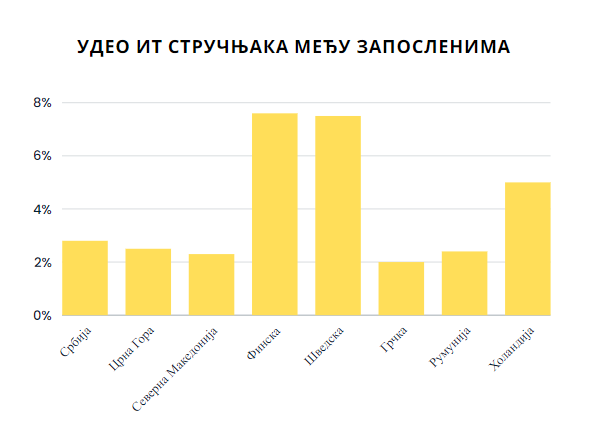
\includegraphics[width=0.8\textwidth, height=7cm]{Slike/radna_snaga.png}
    \end{center}
    \caption{Удео ИТ стручњака међу запосленима \cite{danas_it}.}
    \label{fig:it_evropa}
\end{figure}

\section{Однос полова у информатици на Математичком факултету у Београду}

На основу података, које смо добили са Хипатије\footnote{Факултетски студентски сервис 
Математичког факултета у Београду} можемо уочити да постоји значајна разлика у броју мушких и 
женских студената на смеру Информатика, на Математичком факултету у Београду. Ако погледамо табелу
\ref{tab:tabela1} можемо да закључимо да је ова област постала све популарнија, како у мушком, 
тако и у женском свету и да је однос полава све сличнији. Такође на слици \ref{fig:odnos} 
приказан је однос полова у процентима по годинама. 

\begin{table}[h!]
    \begin{center}
        \caption{\small{Однос полова на Математичком факултету на смеру Информатика.}}
        \Large

        \vspace{10}
        \begin{tabular}{|a|b|c|} \hline
        %centralno poravnanje& levo poravnanje& desno poravnanje\\ \hline
        Година & Мушкарци & Жене\\ \hline
        2015. & 103 & 41 \\ \hline
        2016. & 93  & 52 \\ \hline
        2017. & 132 & 55 \\ \hline
        2018. & 124 & 68 \\ \hline
        2019. & 116 & 79 \\ \hline
        \end{tabular}
        \label{tab:tabela1}
    \end{center}
\end{table}


\begin{figure}[h!]
    \begin{center}
        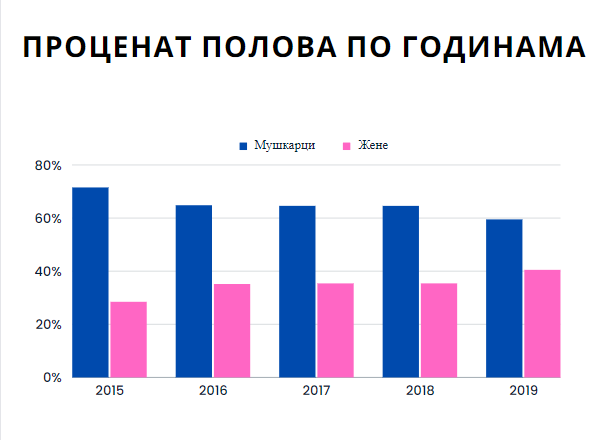
\includegraphics[width=0.8\textwidth, height=7cm]{Slike/odnos_po_godinama.png}
    \end{center}
    \caption{Однос између жена и мушкараца на Математичком факултету у Београду, смер информатика.}
    \label{fig:odnos}
\end{figure}

\section{Заједнице које се баве промовисањем родне равноправности у Србији}

У наредној табели \ref{tab:tabela2} су приказане неке организације у Србији, које се баве и залажу
за родну равноправност.

\begin{table}[h!]
    \begin{center}
        \caption{\small{Преглед неколико заједница које се баве промовисањем родне равноправности у Србији.}}
        
        \vspace{10}
        \begin{tabular}{|a|b|c|} \hline
        %centralno poravnanje& levo poravnanje& desno poravnanje\\ \hline
        Назив &Оснивач &Година оснивања\\ \hline
        Фондација Ана и Владе Дивац  & Ана и Владе Дивац   & 2007 \\  \hline
        Фондација за отворено друштво - Србија   & Џорџ Сорос & 1991 \\ \hline
        Женска платформа за развој Србије & GKH\tablefootnote{GenderKnowledgeHub organizacija} &2016\\ \hline
        \end{tabular}
        \label{tab:tabela2}
    \end{center}
\end{table}

Циљ фондације \textit{"Ана и Владе Дивац"} је пружање пордшке различитим пројектима и иницијативама у области образовања, здравства, социјалне инклузије, спорта и културе у Србији. Фондација \textit{"Ана и Владе Дивац"} заједно са Министарством за бригу о породици, и уз подршку Европске уније, одржала је бројне конференције у циљу пружања помоћи женама у раду, јачањања партнерских односа између запослених и послодаваца, као и информисању о правима из области рада и запошљавања, са посебним акцентом на жене. Имајући у виду да у Србији и даље постоји неравноправност између полова, као и стереотипи када је у питању улога жене у породичном животу, фондација \textit{"Ана и Владе Дивац"} велику пажњу посвећује усклађивању рада и родитељства сваког појединца. Од свих притужби које су стигле поверенику за заштиту равноправности у периоду 2014 - 2018. године на другом месту налазе се притужбе на дискриминацију у области рада и запошљавања. Жене као разлоге најчешће наводе постављање на ниже радне позиције, отказ уговора о раду након повратка са породиљског одсуства, одсуство са посла због бриге о деци, као и године старости. Према подацима Националне стратегије за родну равноправност Републике Србије (2016 – 2020), 95\% свих жена у Србији дневно троши пет сати на кућне послове, док мушкарци троше готово 40\% мање - три сата и имају сат времена више слободног времена него жене. Чак 70\% очева са дететом је успело да напредује у каријери, док је само 30\% жена у истој ситуацији било у могућности да оствари напредак \cite{fondacijaAna}.\\

Фондација за отворено друштво - Србија је део мреже Фондације за отворено друштво (енгл. Open society foundations) са седиштем у Њујорку, једне од највећих филантропских организација у свету. Кроз програм социјална и економска правда, фондација између осталих бројних циљева има за циљ покретање и подржавање иницијативе организација, покрета и активиста посвећених укључивању грађана (жена, Рома, неформалних радника) у шири социјални дијалог и кључне реформске процесе (укључујући процес европских интеграција), како би се зауставила ерозија и унапредило поштовање економских и социјалних права, а посебно права на рад, образовање и здравље \cite{fondacijaVrata}. \\
    
Женска платформа за развој Србије (енгл. GKH) је независни истраживачки центар у области родне равноправности, основан са циљем да допринесе креирању родно одговорних политика и пројеката заснованих на подацима. Ова организација се бави решавањем проблема неправедног и неравномерног дистрибуирања јавних ресурса између мушкараца и жена, као и истраживањем родних односа у различитим областима. Такође бави се и креирањем методологија, база података и различитих алата за праћење равноправности. Циљ платформе јесу спровођење родне анализе, организација различитих курсева, трибина и конференција, које промовишу знање о родној равноправности. На платформи се такође објављују анализе и смернице за увођење родне перспективе \cite{fondacijaZene}. 

\section{Иницијативе које се баве родном равноправношћу у Србији}
\label{sec:naslov3}

Повећање броjа девоjака у ИТ-у важно jе како за девоjке, коjе
треба охрабрити и пружити им подршку да се равноправно укључе у
jедну од наjперспективниjих пословних области, тако и за сам ИТ сектор, 
jер родни диверзитет може значаjно да допринесе jачању читаве индустриjе. 
Међутим, перцепциjа да jе ИТ и даље "мушки свет" jе и
даље широко распострањена. Чак и у компанији Гугл (енгл. Google\footnote{Aмеричка мултинационална 
корпорација специјализирана у интернетским сервисима и производима, који укључују интернетске 
рекламне технологије, претрагу, интернетско складиштење и софтвер.}), која се поноси својим 
прогресивним идеалима и која се бори за диверзитет, тек 20\% инжењера су жене \cite{gugl}. 
Управо са тим циљем настаjу и броjе инициjативе - да охрабре и подрже девоjке 
да започну или наставе кариjеру у том правцу.\\

Честа jе поjава да се девоjке ређе одлучуjу да се приjаве за праксу
или посао. Наjчешћи став jе да нису довољно добре или да нису
спремне па због тога уопште и не покушаваjу. Уочивши оваj проблем,
развоjни центар компаниjе Маjкрософт у Србиjи jе 2014. године започео 
инициjативу "Women know it" са циљем оснаживања жена кроз
приче и искуства оних коjе су већ започеле кариjеру у тоj фирми и
тако им приближе први корак, а то jе приjава за посао у ИТ индустриjи. 
Мисиjа ове инициjативе jесте да охрабре младе девоjке и за
собом повуку нову генерациjу девоjака коjе ће наставити да креираjу
технологиjу будућности. Током овог догађаjа, до сада одржаваног
под називом "Женске приче у ИТ-у", студенткиње и ученице средњих школа имаjу 
прилику да чуjу приче и да се упознаjу са радом не само инжењерки из Мајкрософт 
развојног центра, већ и из других ИТ компанија \cite{microsoft}.\\

Такође, јако је важно радити са децом у најранијем периоду и рушити стереотипе. Постоје 
истраживања која кажу да девојчице губе интересовања за технологиjу већ од шесте 
године, а да се то годинама све више појачава. Начин како се технологија 
представља деци прилагођена је дечацима и њиховим интересовањима. Подстакнуте 
том чињеницом, успешне предузеткиње у Србији покренуле су иницијативу у виду 
новости "Girls \& Tech Weekly", како би прилагодиле технологију девојчицама и 
представиле им тако да њима буде занимљиво. Намењена је родитељима и наставницима 
како би их усмерила како да приступе упознавању девојчица са технологијом на 
интересантан начин. Седмично предлаже различите књиге, филмове, видео снимке, али 
и видове забаве и активности за групе девојчица \cite{girls}.\\

Глобално признат покрет "Lean In", који своје корене има у истоименом бестселеру
"Lean In: Women, Work, and the Will to Lead", има своју верзију и у Србији \cite{lean}. 
Књига и иницијатива истражују теме везане за жене у пословном свету, укључујући изазове 
са којима се суочавају у радном окружењу. За циљ има подстицање жена да преузму
активнију улогу у својој каријери, подстичући их да се више ангажују, преузимају 
иницијативу и усуде тражити више у професионалном свету. Помаже женама да виде 
себе као лидере у свету који им каже да то нису. Централна порука је подстицање 
жена да се активно укључе у професионалне ситуације, граде самопоуздање и траже 
прилике за напредовање.


\subsection{Eugain - European Network For Gender Balance in Informatics}
\label{subsec:podnaslov3}

Жене су недовољно заступљене у информатичким наукама, како у академским 
круговима тако и у индустрији. Главна сврха иницијативе Eugain, настале 2020. 
године, јесте побољшање равнотеже полова у ИТ наукама на свим нивоима \cite{eugain}. Приоритети 
су им да мотивишу девојке да упишу факултет у области информатике, охрабре их 
да успешно започну своју каријеру и подрже у превазилажењу свих препрека које жене 
спречавају да достигну сениорске позиције. У склопу ове иницијативе организоване 
су разноврсне школе, радионице и конференције како би се ширили циљеви и акције и 
унапредила истраживачка сарадња како би идеје могле да се развијају и изван граница. 
Значај се огледа у формирању европске мреже колега који се сви са истим циљевима 
боре у својим земљама и истраживачким заједницама за једнакост полова. Упркос 
свим напорима за промене широм Европе, напредак је и даље спор.

\section{Предности родног диверзитета} 
\label{sec:prednosti}
Зашто је важно да постоје мешовити тимови и диверзитет на извршним позицијама? 
Зашто је потребно оснажити жене у ИТ-у? \\
Промовисање родне равноправности у ИТ индустрији не само да је етички важно, већ придоноси 
одрживости, конкурентности и иновацијама у глобалном пословном окружењу. Глобално истраживањe 
рађено у 21 980 фирми, у 91 држави, показује да нас лош положај жена кошта на више поља.
Компаније у којима жене чине најмање трећину борда имају веће приходе, фирме
које воде предузетнице имају већу финансијску сигурност, а тимови који су предвођени
женама доносе 20\% више иновација \cite{prednosti}. 

Није нужно доказано да су жене боље у вођењу послова, али докази показују да разноликости 
на нивоу доношења одлука помажу. Различите вештине, стилови рада и приступи проблему 
дорпиносе успешнијем решавању изазова. Разноликост не само у погледу пола већ и 
кроз различите културе такође побољшава перформансе компаније \cite{kultura}.\\ 

Присуство различитих перспектива, искустава и идеја доноси богатство иновација, 
повећава се креативност и способност решавања проблема на иновативан начин. 
Логика пословања такође сугерише да је у интересу готово сваке компаније 
ангажoвати најбоље од људског капитала доступног на тржишту рада, прилагодити свој
производ или услугу ширем кругу људи, укључујући и жене и мушкарце, и препознати
потребе својих купаца (на пример жене у САД чешће доносе одлуке о куповини).

\section{Закључак}
\label{sec:zakljucak}

Последице дигитализације у сфери рада на родну равноправност су још увек
недовољно истражена тема, а постојеће студије не дају коначне одговоре на питања као што
су: да ли ће жене надоместити недостајуће ИКТ кадрове, да ли је ризик од аутоматизације
послова већи за жене, итд. 
Проналажење баланса између изазивања и наметања (кроз обавезне предмете) интересовања за ИКТ и 
МИНТ (енгл. STEM\footnote{Енглески појам STEM јавља се као акроним, који 
упућује на неколико академских дисциплина: наука (Science), технологија (Technology), инжењеринг 
(Engineerin) и математика (Mathematics).}), подизање самопоуздања девојака и жена када су у питању
технологије, али и флексибилни радни аранжмани само су неки од фактора, који упућују да
превазилажење родних стереотипа о мушким и женским позивима тражи софистицирани приступ.
То се преноси и на теме изван образовања и рада у ИКТ-у, имајући у виду да рад са дигиталним
технологијама не значи, и у будућности ће све мање значити, искључиво рад у ИКТ-у, па чак и шире
у МИНТ областима. У том контексту разлике у дигиталним вештинама жена и мушкараца
представљају савремени показатељ родног дигиталног јаза. 

Чињеница која охрабрује јесте да међу младима (како у Србији тако и у Европској унији) родне 
разлике изостају. Не треба изоставити то да када данашњи млади буду доминантна радна снага, 
схватање дигиталних вештина (као и одговарајући показатељи) ће се мењати ка способностима за 
разумевање и коришћење комплексијиних елемената попут вештачке интелигенције, машинског учења и 
слично. 

\newpage
\addcontentsline{toc}{section}{Литература}
\appendix
\bibliography{seminarski} 
\bibliographystyle{unsrt}
%\bibliographystyle{plain}

\end{document}
